\documentclass[12pt]{scrartcl}

\usepackage[utf8]{inputenc}
\usepackage[T1]{fontenc}
\usepackage{lmodern}
\usepackage{graphicx}
%\usepackage[pdftex,hyperref,dvipsnames]{xcolor}
\usepackage{listings}
\usepackage[a4paper,lmargin={2cm},rmargin={2cm},tmargin={3.5cm},bmargin = {2.5cm},headheight = {4cm}]{geometry}
\usepackage{amsmath,amssymb,amstext,amsthm}
% \usepackage[lined,algonl,boxed]{algorithm2e} 
%\usepackage{algpseudocode}
\usepackage{tikz}
\usepackage{pgfplots}
\usepackage{url}
\usepackage{tcolorbox}
\usepackage[inline]{enumitem}
\usepackage[headsepline]{scrlayer-scrpage} 
\usepackage{float}

\usepackage[scale=0.55, lineVdist=1em]{secstack}
\pagestyle{scrheadings} 
\usetikzlibrary{automata,positioning}
\graphicspath{ {./images/} }

\usepgfplotslibrary{external}
%\tikzexternalize
\pgfplotsset{width=10cm,compat=1.9}
\pgfplotsset{every axis/.style={
    axis line style = thick,
    grid = both,
    tick pos = left,
    tick align = outside,
    tick style = {thick,black},
    fill = blue,
	line width = 2pt,
}}

\lstset{
  basicstyle=\ttfamily\small,
  numbers=left,
  numberstyle=\tiny,
  stepnumber=1,
  numbersep=8pt,
  frame=single,
  breaklines=true,
  columns=fullflexible
}

\lstset{
  language=C,
  basicstyle=\ttfamily\small,
  keywordstyle=\color{blue},
  commentstyle=\color{gray},
  stringstyle=\color{green!60!black},
  numbers=left,
  numberstyle=\tiny,
  stepnumber=1,
  numbersep=8pt,
  frame=single,
  breaklines=true,
  columns=fullflexible
}

\renewcommand{\theenumi}{(\alph{enumi})}
\renewcommand{\labelenumi}{\text{\theenumi}}
\renewcommand{\labelenumii}{(\roman{enumii})} 

\ohead{Marvin Simon (3883376)\\
       Jan Theil (3794698)}

\ihead{System and Web Security}

\newcounter{exnum}
\newcommand{\exercise}[1]{\section*{Problem \theexnum\stepcounter{exnum}: #1}}

\begin{document}

\setcounter{exnum}{1}
\exercise{Stack-based Overflow}
We are calling the program \textit{sof-exploit-10.c} with our exploit program and feeding it argument parameters which are overwriting the buffer of the local variable \verb|b|.

We then set the return address to some address in our local \verb|b|. We filled the variable \verb|b| with nops and the shellcode execution. So now we only need to hit one of the NOPS and it executes the injected shellcode.


\begin{figure}[H]
    \centering
    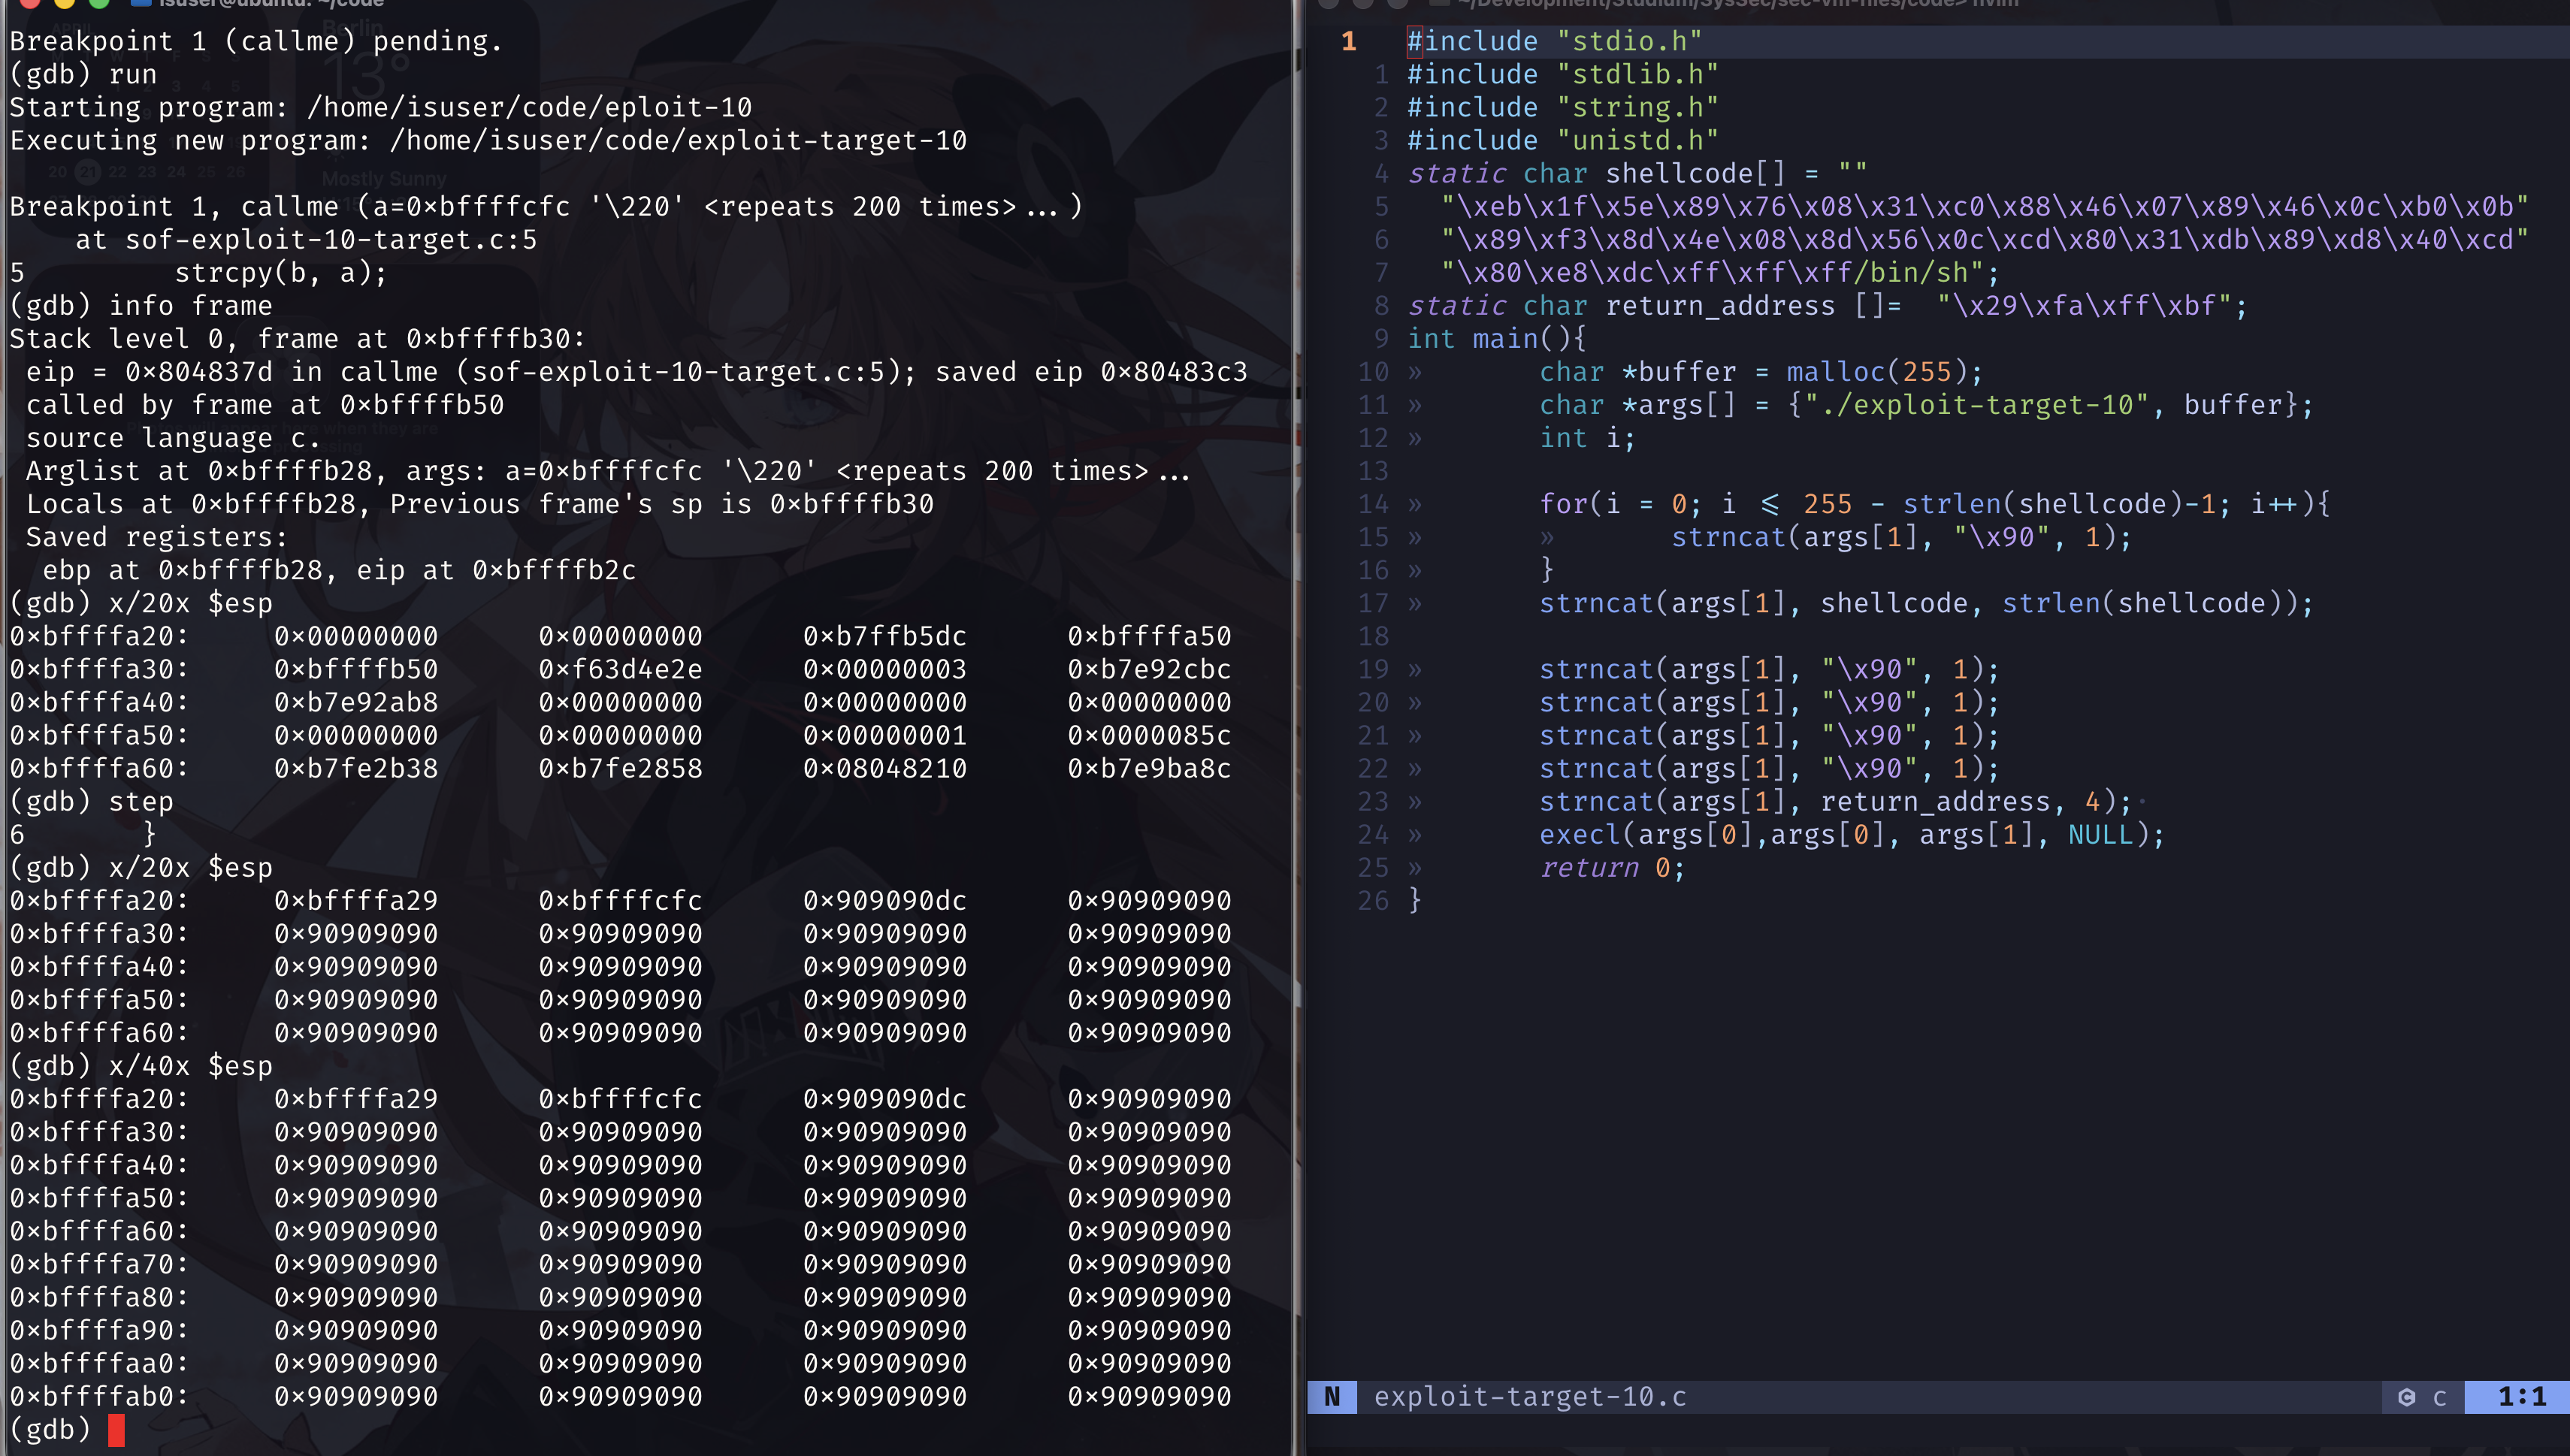
\includegraphics[width=\textwidth]{Attack_Screenshot_1.png}
    \caption{Finding out the return address within \texttt{b}}
    \label{fig:Attack_Screenshot_1}
\end{figure}

\begin{figure}[H]
    \centering
    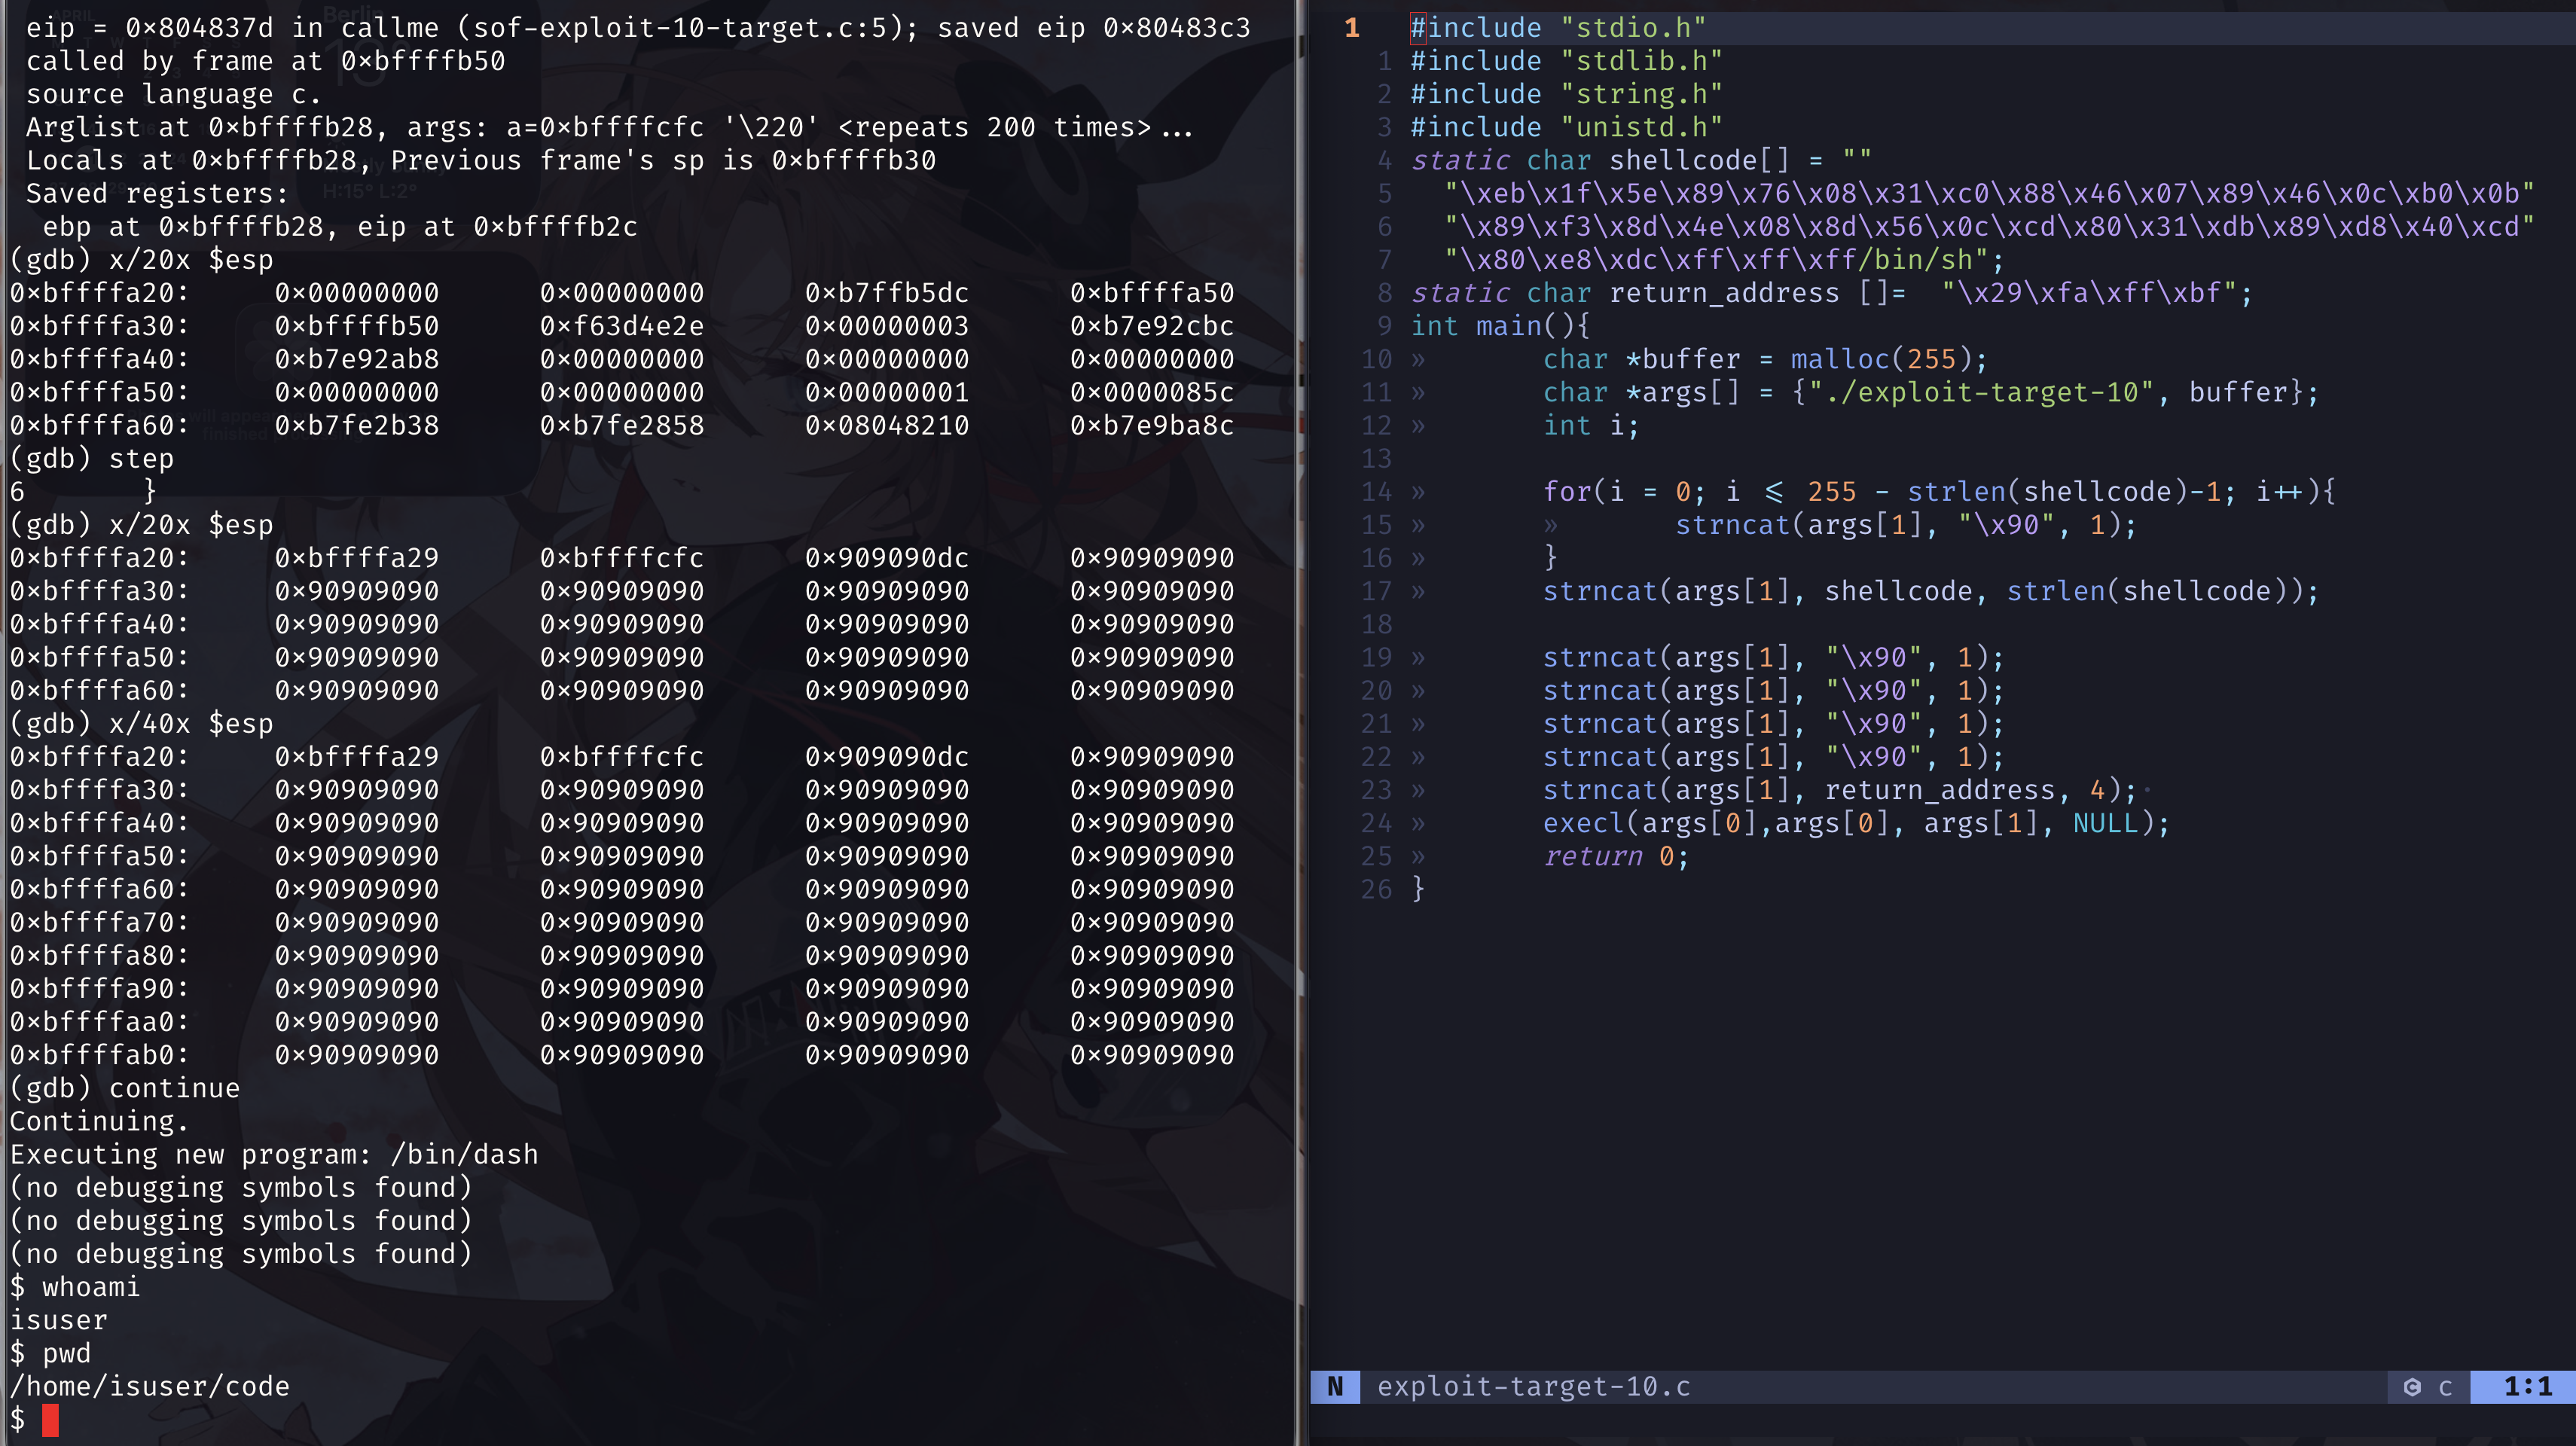
\includegraphics[width=\textwidth]{Attack_Screenshot_2.png}
    \caption{Running the attack}
    \label{fig:Attack_Screenshot_2}
\end{figure}

\exercise{Stack-based Overflow}
\exercise{Stack-based Overflow}
\exercise{Stack-based Overflow}
\exercise{Memory Alignment}
\end{document}
